\documentclass[twoside]{book}

% Packages required by doxygen
\usepackage{fixltx2e}
\usepackage{calc}
\usepackage{doxygen}
\usepackage[export]{adjustbox} % also loads graphicx
\usepackage{graphicx}
\usepackage[utf8]{inputenc}
\usepackage{makeidx}
\usepackage{multicol}
\usepackage{multirow}
\PassOptionsToPackage{warn}{textcomp}
\usepackage{textcomp}
\usepackage[nointegrals]{wasysym}
\usepackage[table]{xcolor}

% Font selection
\usepackage[T1]{fontenc}
\usepackage[scaled=.90]{helvet}
\usepackage{courier}
\usepackage{amssymb}
\usepackage{sectsty}
\renewcommand{\familydefault}{\sfdefault}
\allsectionsfont{%
  \fontseries{bc}\selectfont%
  \color{darkgray}%
}
\renewcommand{\DoxyLabelFont}{%
  \fontseries{bc}\selectfont%
  \color{darkgray}%
}
\newcommand{\+}{\discretionary{\mbox{\scriptsize$\hookleftarrow$}}{}{}}

% Page & text layout
\usepackage{geometry}
\geometry{%
  a4paper,%
  top=2.5cm,%
  bottom=2.5cm,%
  left=2.5cm,%
  right=2.5cm%
}
\tolerance=750
\hfuzz=15pt
\hbadness=750
\setlength{\emergencystretch}{15pt}
\setlength{\parindent}{0cm}
\setlength{\parskip}{0.2cm}
\makeatletter
\renewcommand{\paragraph}{%
  \@startsection{paragraph}{4}{0ex}{-1.0ex}{1.0ex}{%
    \normalfont\normalsize\bfseries\SS@parafont%
  }%
}
\renewcommand{\subparagraph}{%
  \@startsection{subparagraph}{5}{0ex}{-1.0ex}{1.0ex}{%
    \normalfont\normalsize\bfseries\SS@subparafont%
  }%
}
\makeatother

% Headers & footers
\usepackage{fancyhdr}
\pagestyle{fancyplain}
\fancyhead[LE]{\fancyplain{}{\bfseries\thepage}}
\fancyhead[CE]{\fancyplain{}{}}
\fancyhead[RE]{\fancyplain{}{\bfseries\leftmark}}
\fancyhead[LO]{\fancyplain{}{\bfseries\rightmark}}
\fancyhead[CO]{\fancyplain{}{}}
\fancyhead[RO]{\fancyplain{}{\bfseries\thepage}}
\fancyfoot[LE]{\fancyplain{}{}}
\fancyfoot[CE]{\fancyplain{}{}}
\fancyfoot[RE]{\fancyplain{}{\bfseries\scriptsize Generated on Sat Jun 6 2015 21\+:45\+:42 for Anomaly\+Detection\+N\+S3 by Doxygen }}
\fancyfoot[LO]{\fancyplain{}{\bfseries\scriptsize Generated on Sat Jun 6 2015 21\+:45\+:42 for Anomaly\+Detection\+N\+S3 by Doxygen }}
\fancyfoot[CO]{\fancyplain{}{}}
\fancyfoot[RO]{\fancyplain{}{}}
\renewcommand{\footrulewidth}{0.4pt}
\renewcommand{\chaptermark}[1]{%
  \markboth{#1}{}%
}
\renewcommand{\sectionmark}[1]{%
  \markright{\thesection\ #1}%
}

% Indices & bibliography
\usepackage{natbib}
\usepackage[titles]{tocloft}
\setcounter{tocdepth}{3}
\setcounter{secnumdepth}{5}
\makeindex

% Hyperlinks (required, but should be loaded last)
\usepackage{ifpdf}
\ifpdf
  \usepackage[pdftex,pagebackref=true]{hyperref}
\else
  \usepackage[ps2pdf,pagebackref=true]{hyperref}
\fi
\hypersetup{%
  colorlinks=true,%
  linkcolor=blue,%
  citecolor=blue,%
  unicode%
}

% Custom commands
\newcommand{\clearemptydoublepage}{%
  \newpage{\pagestyle{empty}\cleardoublepage}%
}


%===== C O N T E N T S =====

\begin{document}

% Titlepage & ToC
\hypersetup{pageanchor=false,
             bookmarks=true,
             bookmarksnumbered=true,
             pdfencoding=unicode
            }
\pagenumbering{roman}
\begin{titlepage}
\vspace*{7cm}
\begin{center}%
{\Large Anomaly\+Detection\+N\+S3 }\\
\vspace*{1cm}
{\large Generated by Doxygen 1.8.9.1}\\
\vspace*{0.5cm}
{\small Sat Jun 6 2015 21:45:42}\\
\end{center}
\end{titlepage}
\clearemptydoublepage
\tableofcontents
\clearemptydoublepage
\pagenumbering{arabic}
\hypersetup{pageanchor=true}

%--- Begin generated contents ---
\chapter{Hierarchical Index}
\section{Class Hierarchy}
This inheritance list is sorted roughly, but not completely, alphabetically\+:\begin{DoxyCompactList}
\item \contentsline{section}{ns3\+:\+:Data\+Source}{\pageref{classns3_1_1DataSource}}{}
\item \contentsline{section}{ns3\+:\+:Detector}{\pageref{classns3_1_1Detector}}{}
\begin{DoxyCompactList}
\item \contentsline{section}{ns3\+:\+:Detector\+Euclidean}{\pageref{classns3_1_1DetectorEuclidean}}{}
\end{DoxyCompactList}
\item \contentsline{section}{ns3\+:\+:Matrix}{\pageref{classns3_1_1Matrix}}{}
\item \contentsline{section}{ns3\+:\+:Model}{\pageref{classns3_1_1Model}}{}
\begin{DoxyCompactList}
\item \contentsline{section}{ns3\+:\+:Euclidean\+Model}{\pageref{classns3_1_1EuclideanModel}}{}
\end{DoxyCompactList}
\item \contentsline{section}{ns3\+:\+:Result}{\pageref{structns3_1_1Result}}{}
\end{DoxyCompactList}

\chapter{Class Index}
\section{Class List}
Here are the classes, structs, unions and interfaces with brief descriptions\+:\begin{DoxyCompactList}
\item\contentsline{section}{\hyperlink{classDataSource}{Data\+Source} \\*Abstract class of \hyperlink{classDataSource}{Data\+Source} }{\pageref{classDataSource}}{}
\item\contentsline{section}{\hyperlink{classDetector}{Detector} \\*Abstract class of \hyperlink{classDetector}{Detector} }{\pageref{classDetector}}{}
\item\contentsline{section}{\hyperlink{classDetectorEuclidean}{Detector\+Euclidean} \\*Euclidian detector used for the 1st algorithm for A\+D Inherit from \hyperlink{classDetector}{Detector} }{\pageref{classDetectorEuclidean}}{}
\item\contentsline{section}{\hyperlink{classEuclideanModel}{Euclidean\+Model} \\*Euclidian model for the 1st algorithm for A\+D Inherit from \hyperlink{classModel}{Model} }{\pageref{classEuclideanModel}}{}
\item\contentsline{section}{\hyperlink{classMatrix}{Matrix} \\*Tool class used for manipulate data from input data and features }{\pageref{classMatrix}}{}
\item\contentsline{section}{\hyperlink{classModel}{Model} \\*Abstract class of \hyperlink{classModel}{Model} }{\pageref{classModel}}{}
\item\contentsline{section}{\hyperlink{structResult}{Result} }{\pageref{structResult}}{}
\end{DoxyCompactList}

\chapter{File Index}
\section{File List}
Here is a list of all documented files with brief descriptions\+:\begin{DoxyCompactList}
\item\contentsline{section}{\hyperlink{ads-simulator_8cc}{ads-\/simulator.\+cc} \\*File containing the A\+D detector and simulation This file contains both headers and declarations for classes + run the simulator in the main class (instead of classic couple .h and .cc because I need to understand the setup to do so in N\+S3 (act as module or similar with wscript) }{\pageref{ads-simulator_8cc}}{}
\end{DoxyCompactList}

\chapter{Class Documentation}
\hypertarget{classDataSource}{}\section{Data\+Source Class Reference}
\label{classDataSource}\index{Data\+Source@{Data\+Source}}


Abstract class of \hyperlink{classDataSource}{Data\+Source}.  


\subsection*{Public Member Functions}
\begin{DoxyCompactItemize}
\item 
\hypertarget{classDataSource_a3c50a75418afefcc1e57577c033c6678}{}virtual \hyperlink{classMatrix}{Matrix} $\ast$ {\bfseries Extract\+Sample\+Features} ()=0\label{classDataSource_a3c50a75418afefcc1e57577c033c6678}

\item 
\hypertarget{classDataSource_a2001cf0cb5718df33bfe83607e56057b}{}virtual double $\ast$ {\bfseries Extract\+Features} (Ptr$<$ Packet $>$ packet)=0\label{classDataSource_a2001cf0cb5718df33bfe83607e56057b}

\item 
\hypertarget{classDataSource_ae4f3eda38c1c60f0dbfe56dc0199f5e3}{}virtual void {\bfseries Update\+Data\+Base} (double $\ast$features)=0\label{classDataSource_ae4f3eda38c1c60f0dbfe56dc0199f5e3}

\item 
\hypertarget{classDataSource_a50bf1acad05cf5db970319524f503be7}{}virtual uint16\+\_\+t {\bfseries Get\+Number\+Features} ()\label{classDataSource_a50bf1acad05cf5db970319524f503be7}

\end{DoxyCompactItemize}
\subsection*{Protected Attributes}
\begin{DoxyCompactItemize}
\item 
\hypertarget{classDataSource_a71c41d9d7d6cfdd4db0e0176a24f0521}{}uint16\+\_\+t {\bfseries m\+\_\+num\+\_\+features}\label{classDataSource_a71c41d9d7d6cfdd4db0e0176a24f0521}

\end{DoxyCompactItemize}


\subsection{Detailed Description}
Abstract class of \hyperlink{classDataSource}{Data\+Source}. 

The documentation for this class was generated from the following file\+:\begin{DoxyCompactItemize}
\item 
\hyperlink{ads-simulator_8cc}{ads-\/simulator.\+cc}\end{DoxyCompactItemize}

\hypertarget{classDetector}{}\section{Detector Class Reference}
\label{classDetector}\index{Detector@{Detector}}


Abstract class of \hyperlink{classDetector}{Detector}.  


Inheritance diagram for Detector\+:\begin{figure}[H]
\begin{center}
\leavevmode
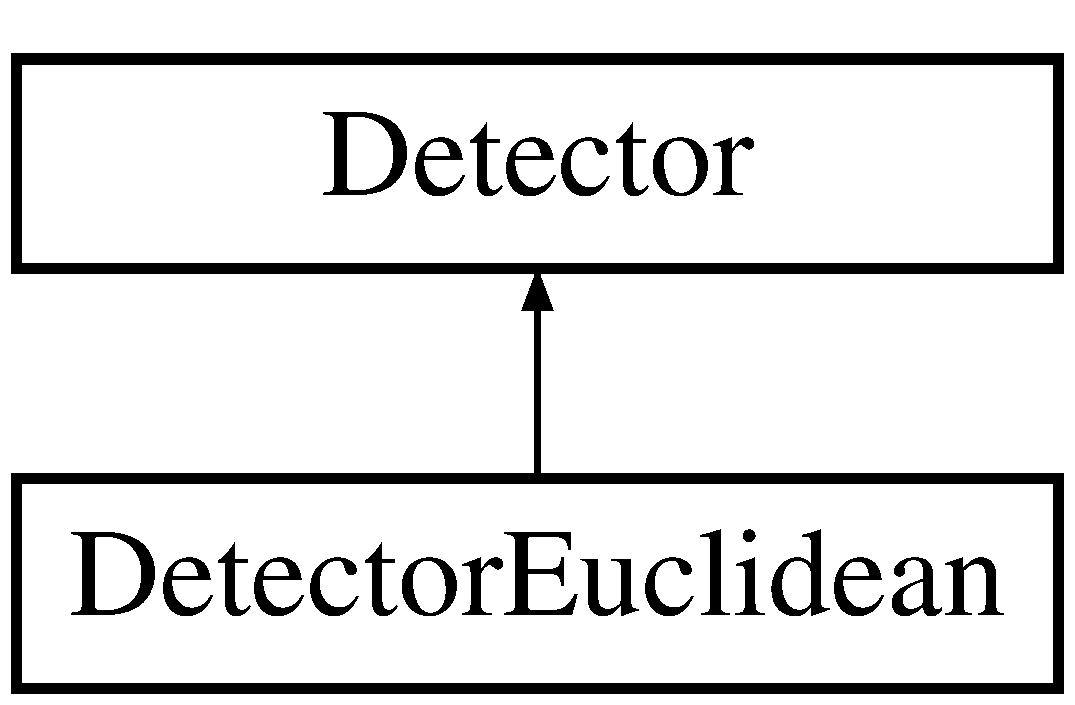
\includegraphics[height=2.000000cm]{classDetector}
\end{center}
\end{figure}
\subsection*{Public Member Functions}
\begin{DoxyCompactItemize}
\item 
\hypertarget{classDetector_ad1eaa0403bdfc31b523fc7ee837bd2e6}{}{\bfseries Detector} (\hyperlink{classDataSource}{Data\+Source} $\ast$ds, \hyperlink{classModel}{Model} $\ast$m, uint64\+\_\+t p\+\_\+init, uint64\+\_\+t p\+\_\+train\+\_\+interval, bool p\+\_\+only\+\_\+one\+\_\+train)\label{classDetector_ad1eaa0403bdfc31b523fc7ee837bd2e6}

\item 
\hypertarget{classDetector_ab791196650bf084ead62c88d29b6ef53}{}{\bfseries Detector} (\hyperlink{classDataSource}{Data\+Source} $\ast$ds, uint64\+\_\+t p\+\_\+init, uint64\+\_\+t p\+\_\+train\+\_\+interval, bool p\+\_\+only\+\_\+one\+\_\+train)\label{classDetector_ab791196650bf084ead62c88d29b6ef53}

\item 
\hypertarget{classDetector_a0b509e253c05cb27135524c4a7812c30}{}virtual \hyperlink{structResult}{Result} {\bfseries Evaluate} ()=0\label{classDetector_a0b509e253c05cb27135524c4a7812c30}

\item 
\hypertarget{classDetector_a25534c5a1eefeae99b3cfa1cc2c560ca}{}virtual void {\bfseries Train} (bool anomaly)=0\label{classDetector_a25534c5a1eefeae99b3cfa1cc2c560ca}

\item 
\hypertarget{classDetector_aedc62b2e44f9ade929695432abe49279}{}void {\bfseries register\+Feature\+Extractor} (\hyperlink{classDataSource}{Data\+Source} $\ast$datasource)\label{classDetector_aedc62b2e44f9ade929695432abe49279}

\end{DoxyCompactItemize}
\subsection*{Protected Attributes}
\begin{DoxyCompactItemize}
\item 
\hypertarget{classDetector_a8a5e1748b785cfca369357a80f85fdc3}{}\hyperlink{classDataSource}{Data\+Source} $\ast$ {\bfseries m\+\_\+datasource}\label{classDetector_a8a5e1748b785cfca369357a80f85fdc3}

\item 
\hypertarget{classDetector_a7848ee9218c0b91632acd45180db1c31}{}\hyperlink{classModel}{Model} $\ast$ {\bfseries m\+\_\+model}\label{classDetector_a7848ee9218c0b91632acd45180db1c31}

\item 
\hypertarget{classDetector_a025d23b856701f341fbc4067457fc907}{}uint64\+\_\+t {\bfseries m\+\_\+init\+\_\+period}\label{classDetector_a025d23b856701f341fbc4067457fc907}

\item 
\hypertarget{classDetector_ab5187390b9fe4d8794517c4611c91044}{}uint64\+\_\+t {\bfseries m\+\_\+train\+\_\+interval}\label{classDetector_ab5187390b9fe4d8794517c4611c91044}

\item 
\hypertarget{classDetector_add0d08bdaa26cd6c81710da5d4be4b84}{}bool {\bfseries m\+\_\+only\+\_\+one\+\_\+train}\label{classDetector_add0d08bdaa26cd6c81710da5d4be4b84}

\end{DoxyCompactItemize}


\subsection{Detailed Description}
Abstract class of \hyperlink{classDetector}{Detector}. 

The documentation for this class was generated from the following file\+:\begin{DoxyCompactItemize}
\item 
\hyperlink{ads-simulator_8cc}{ads-\/simulator.\+cc}\end{DoxyCompactItemize}

\hypertarget{classDetectorEuclidean}{}\section{Detector\+Euclidean Class Reference}
\label{classDetectorEuclidean}\index{Detector\+Euclidean@{Detector\+Euclidean}}


Euclidian detector used for the 1st algorithm for A\+D Inherit from \hyperlink{classDetector}{Detector}.  


Inheritance diagram for Detector\+Euclidean\+:\begin{figure}[H]
\begin{center}
\leavevmode
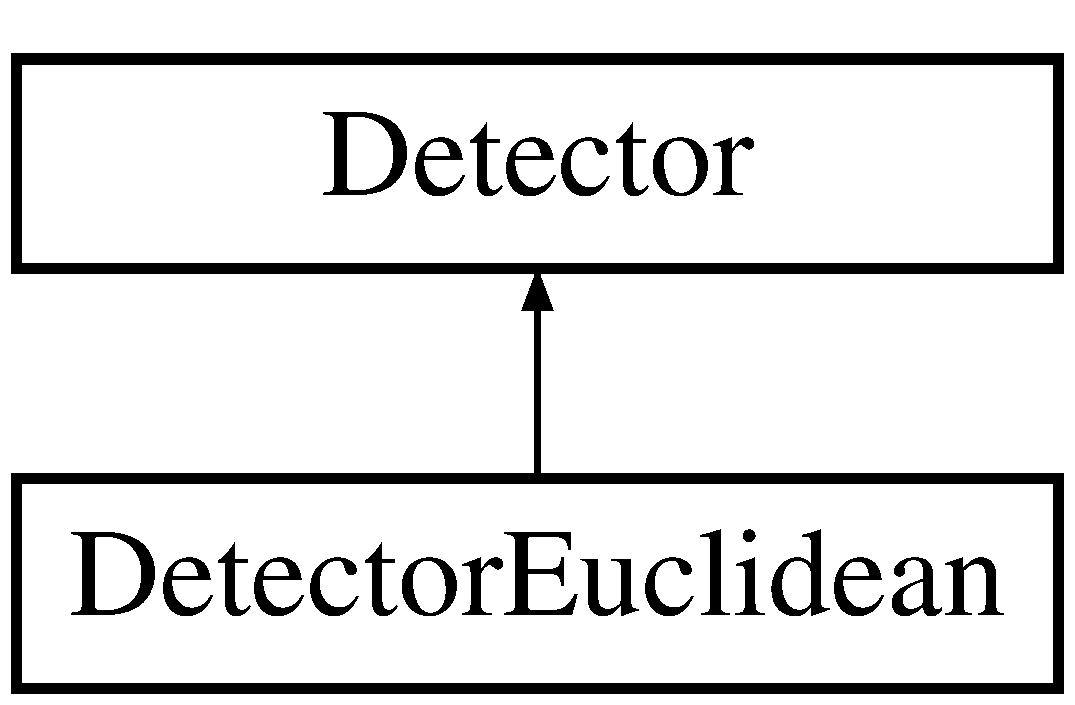
\includegraphics[height=2.000000cm]{classDetectorEuclidean}
\end{center}
\end{figure}
\subsection*{Public Member Functions}
\begin{DoxyCompactItemize}
\item 
\hypertarget{classDetectorEuclidean_a2a7588db4d1b5ddad59ad75ff044dfa2}{}{\bfseries Detector\+Euclidean} (\hyperlink{classDataSource}{Data\+Source} $\ast$ds, Ptr$<$ Node $>$ p\+\_\+node, \hyperlink{classModel}{Model} $\ast$m, uint64\+\_\+t p\+\_\+init, uint64\+\_\+t p\+\_\+train\+\_\+interval, bool p\+\_\+only\+\_\+one\+\_\+train, bool p\+\_\+norm\+\_\+data, bool p\+\_\+time\+\_\+ref)\label{classDetectorEuclidean_a2a7588db4d1b5ddad59ad75ff044dfa2}

\item 
\hyperlink{classDetectorEuclidean_acf39a526724307f8ceb9c3c4cc7550a8}{Detector\+Euclidean} (\hyperlink{classDataSource}{Data\+Source} $\ast$ds, Ptr$<$ Node $>$ p\+\_\+node, uint64\+\_\+t p\+\_\+init, uint64\+\_\+t p\+\_\+train\+\_\+interval, bool p\+\_\+only\+\_\+one\+\_\+train, bool p\+\_\+norm\+\_\+data, bool p\+\_\+time\+\_\+ref)
\item 
\hyperlink{classDetectorEuclidean_ab148b531d1c0ae8b459b6d42bf3b2221}{$\sim$\+Detector\+Euclidean} ()
\item 
\hyperlink{structResult}{Result} \hyperlink{classDetectorEuclidean_aa6dd14b9caad9b551aae97db2b52655f}{Evaluate} ()
\item 
void \hyperlink{classDetectorEuclidean_ab925bf1423f99478e3b57727ade60940}{Train} (bool anomaly)
\item 
\hypertarget{classDetectorEuclidean_a53cfe152d162e3c3dade24c5ac1e6d5f}{}void {\bfseries Open\+Log\+Files} ()\label{classDetectorEuclidean_a53cfe152d162e3c3dade24c5ac1e6d5f}

\item 
\hypertarget{classDetectorEuclidean_a80d5ebd3be8346aefc1d9aabef6963c9}{}void {\bfseries Close\+Log\+Files} ()\label{classDetectorEuclidean_a80d5ebd3be8346aefc1d9aabef6963c9}

\item 
\hypertarget{classDetectorEuclidean_a78fb0e7a0130a2d9124b85000becac3a}{}void {\bfseries Log\+Features} (double $\ast$features, int num\+\_\+features)\label{classDetectorEuclidean_a78fb0e7a0130a2d9124b85000becac3a}

\item 
\hypertarget{classDetectorEuclidean_a56459a2dfe4bd7127c42cb078431f33e}{}void {\bfseries Log\+Norm\+Features} (double $\ast$features, int num\+\_\+features)\label{classDetectorEuclidean_a56459a2dfe4bd7127c42cb078431f33e}

\item 
\hypertarget{classDetectorEuclidean_a832df34bd506af4778ad99b51c3dc909}{}void {\bfseries Log\+Evaluation\+Result} (string packet\+\_\+id, double distance, double threshold, double result, double $\ast$log\+\_\+dst, int num\+\_\+features, Attack\+Type attack)\label{classDetectorEuclidean_a832df34bd506af4778ad99b51c3dc909}

\item 
\hypertarget{classDetectorEuclidean_a467a43419abe69be5d98767aef14c208}{}void {\bfseries Log\+Vector\+Projections} (double $\ast$projections, int size)\label{classDetectorEuclidean_a467a43419abe69be5d98767aef14c208}

\item 
\hypertarget{classDetectorEuclidean_ae2cef48b2e6e5ea6b7f201b7c6a6e27a}{}void {\bfseries Create\+Normality\+Model} ()\label{classDetectorEuclidean_ae2cef48b2e6e5ea6b7f201b7c6a6e27a}

\item 
void \hyperlink{classDetectorEuclidean_a09a0f75f67c2f09560428cef82ff4059}{Update\+Threshold} (\hyperlink{classEuclideanModel}{Euclidean\+Model} $\ast$model, double $\ast$p\+\_\+features, uint16\+\_\+t p\+\_\+num\+\_\+feat, bool p\+\_\+norm\+\_\+data)
\item 
void \hyperlink{classDetectorEuclidean_a5c153476961363c67cf34f467aa06062}{Calculate\+Threshold} (\hyperlink{classEuclideanModel}{Euclidean\+Model} $\ast$model)
\item 
double \hyperlink{classDetectorEuclidean_abed09af9d25d97db2c22546c576de054}{Distance} (double $\ast$v\+\_\+avg\+\_\+feat, double $\ast$v\+\_\+feat, int size, double $\ast$log\+\_\+dst)
\item 
void \hyperlink{classDetectorEuclidean_afaebdff052eee6bbdfabd474f2f3b623}{Update\+Average\+Max\+Min} (\hyperlink{classEuclideanModel}{Euclidean\+Model} $\ast$p\+\_\+inc\+\_\+model, double $\ast$p\+\_\+features, uint16\+\_\+t p\+\_\+num\+\_\+feat)
\item 
void \hyperlink{classDetectorEuclidean_a2507d55c396e0912aa8cc54cded8d9e2}{Calculate\+Average} (\hyperlink{classEuclideanModel}{Euclidean\+Model} $\ast$p\+\_\+inc\+\_\+model, uint16\+\_\+t p\+\_\+num\+\_\+feat, bool p\+\_\+norm\+\_\+data)
\item 
void \hyperlink{classDetectorEuclidean_ac6c5aeafe7ea87499b31169fcbf5a0a1}{Normalise} (double $\ast$max, double $\ast$min, double $\ast$vector, int num\+\_\+elements)
\end{DoxyCompactItemize}
\subsection*{Additional Inherited Members}


\subsection{Detailed Description}
Euclidian detector used for the 1st algorithm for A\+D Inherit from \hyperlink{classDetector}{Detector}. 

\subsection{Constructor \& Destructor Documentation}
\hypertarget{classDetectorEuclidean_acf39a526724307f8ceb9c3c4cc7550a8}{}\index{Detector\+Euclidean@{Detector\+Euclidean}!Detector\+Euclidean@{Detector\+Euclidean}}
\index{Detector\+Euclidean@{Detector\+Euclidean}!Detector\+Euclidean@{Detector\+Euclidean}}
\subsubsection[{Detector\+Euclidean}]{\setlength{\rightskip}{0pt plus 5cm}Detector\+Euclidean\+::\+Detector\+Euclidean (
\begin{DoxyParamCaption}
\item[{{\bf Data\+Source} $\ast$}]{ds, }
\item[{Ptr$<$ Node $>$}]{p\+\_\+node, }
\item[{uint64\+\_\+t}]{p\+\_\+init, }
\item[{uint64\+\_\+t}]{p\+\_\+train\+\_\+interval, }
\item[{bool}]{p\+\_\+only\+\_\+one\+\_\+train, }
\item[{bool}]{p\+\_\+norm\+\_\+data, }
\item[{bool}]{p\+\_\+time\+\_\+ref}
\end{DoxyParamCaption}
)}\label{classDetectorEuclidean_acf39a526724307f8ceb9c3c4cc7550a8}
Anomaly detector\+: Deviation from sum of squared differences It creates the normality model in two steps. First calculates the averages of the features and secondly calculates the threshold used for the distances. \hypertarget{classDetectorEuclidean_ab148b531d1c0ae8b459b6d42bf3b2221}{}\index{Detector\+Euclidean@{Detector\+Euclidean}!````~Detector\+Euclidean@{$\sim$\+Detector\+Euclidean}}
\index{````~Detector\+Euclidean@{$\sim$\+Detector\+Euclidean}!Detector\+Euclidean@{Detector\+Euclidean}}
\subsubsection[{$\sim$\+Detector\+Euclidean}]{\setlength{\rightskip}{0pt plus 5cm}Detector\+Euclidean\+::$\sim$\+Detector\+Euclidean (
\begin{DoxyParamCaption}
{}
\end{DoxyParamCaption}
)}\label{classDetectorEuclidean_ab148b531d1c0ae8b459b6d42bf3b2221}
Destructor for \hyperlink{classDetectorEuclidean}{Detector\+Euclidean} class 

\subsection{Member Function Documentation}
\hypertarget{classDetectorEuclidean_a2507d55c396e0912aa8cc54cded8d9e2}{}\index{Detector\+Euclidean@{Detector\+Euclidean}!Calculate\+Average@{Calculate\+Average}}
\index{Calculate\+Average@{Calculate\+Average}!Detector\+Euclidean@{Detector\+Euclidean}}
\subsubsection[{Calculate\+Average}]{\setlength{\rightskip}{0pt plus 5cm}void Detector\+Euclidean\+::\+Calculate\+Average (
\begin{DoxyParamCaption}
\item[{{\bf Euclidean\+Model} $\ast$}]{p\+\_\+inc\+\_\+model, }
\item[{uint16\+\_\+t}]{p\+\_\+num\+\_\+feat, }
\item[{bool}]{p\+\_\+norm\+\_\+data}
\end{DoxyParamCaption}
)}\label{classDetectorEuclidean_a2507d55c396e0912aa8cc54cded8d9e2}
Method that calculates final average vector. \hypertarget{classDetectorEuclidean_a5c153476961363c67cf34f467aa06062}{}\index{Detector\+Euclidean@{Detector\+Euclidean}!Calculate\+Threshold@{Calculate\+Threshold}}
\index{Calculate\+Threshold@{Calculate\+Threshold}!Detector\+Euclidean@{Detector\+Euclidean}}
\subsubsection[{Calculate\+Threshold}]{\setlength{\rightskip}{0pt plus 5cm}void Detector\+Euclidean\+::\+Calculate\+Threshold (
\begin{DoxyParamCaption}
\item[{{\bf Euclidean\+Model} $\ast$}]{model}
\end{DoxyParamCaption}
)}\label{classDetectorEuclidean_a5c153476961363c67cf34f467aa06062}
Calculate the threshold used to evaluate the distance. \hypertarget{classDetectorEuclidean_abed09af9d25d97db2c22546c576de054}{}\index{Detector\+Euclidean@{Detector\+Euclidean}!Distance@{Distance}}
\index{Distance@{Distance}!Detector\+Euclidean@{Detector\+Euclidean}}
\subsubsection[{Distance}]{\setlength{\rightskip}{0pt plus 5cm}double Detector\+Euclidean\+::\+Distance (
\begin{DoxyParamCaption}
\item[{double $\ast$}]{v\+\_\+1, }
\item[{double $\ast$}]{v\+\_\+2, }
\item[{int}]{size, }
\item[{double $\ast$}]{log\+\_\+dst}
\end{DoxyParamCaption}
)}\label{classDetectorEuclidean_abed09af9d25d97db2c22546c576de054}
Calculate distance between two vectors based on sum of squared differences. \hypertarget{classDetectorEuclidean_aa6dd14b9caad9b551aae97db2b52655f}{}\index{Detector\+Euclidean@{Detector\+Euclidean}!Evaluate@{Evaluate}}
\index{Evaluate@{Evaluate}!Detector\+Euclidean@{Detector\+Euclidean}}
\subsubsection[{Evaluate}]{\setlength{\rightskip}{0pt plus 5cm}{\bf Result} Detector\+Euclidean\+::\+Evaluate (
\begin{DoxyParamCaption}
{}
\end{DoxyParamCaption}
)\hspace{0.3cm}{\ttfamily [virtual]}}\label{classDetectorEuclidean_aa6dd14b9caad9b551aae97db2b52655f}
Function that evaluates the current observation against the normality model.

Returns\+: 0 -\/ Normal evaluation 1 -\/ Abnormal evaluation 

Implements \hyperlink{classDetector}{Detector}.

\hypertarget{classDetectorEuclidean_ac6c5aeafe7ea87499b31169fcbf5a0a1}{}\index{Detector\+Euclidean@{Detector\+Euclidean}!Normalise@{Normalise}}
\index{Normalise@{Normalise}!Detector\+Euclidean@{Detector\+Euclidean}}
\subsubsection[{Normalise}]{\setlength{\rightskip}{0pt plus 5cm}void Detector\+Euclidean\+::\+Normalise (
\begin{DoxyParamCaption}
\item[{double $\ast$}]{max, }
\item[{double $\ast$}]{min, }
\item[{double $\ast$}]{vector, }
\item[{int}]{num\+\_\+elements}
\end{DoxyParamCaption}
)}\label{classDetectorEuclidean_ac6c5aeafe7ea87499b31169fcbf5a0a1}
Method to normalise a vector. \hypertarget{classDetectorEuclidean_ab925bf1423f99478e3b57727ade60940}{}\index{Detector\+Euclidean@{Detector\+Euclidean}!Train@{Train}}
\index{Train@{Train}!Detector\+Euclidean@{Detector\+Euclidean}}
\subsubsection[{Train}]{\setlength{\rightskip}{0pt plus 5cm}void Detector\+Euclidean\+::\+Train (
\begin{DoxyParamCaption}
\item[{bool}]{anomaly}
\end{DoxyParamCaption}
)\hspace{0.3cm}{\ttfamily [virtual]}}\label{classDetectorEuclidean_ab925bf1423f99478e3b57727ade60940}
Method that coordinates the training of the normality model.

Behaviour\+: Creates only one model after an initial period collecting data. 

Implements \hyperlink{classDetector}{Detector}.

\hypertarget{classDetectorEuclidean_afaebdff052eee6bbdfabd474f2f3b623}{}\index{Detector\+Euclidean@{Detector\+Euclidean}!Update\+Average\+Max\+Min@{Update\+Average\+Max\+Min}}
\index{Update\+Average\+Max\+Min@{Update\+Average\+Max\+Min}!Detector\+Euclidean@{Detector\+Euclidean}}
\subsubsection[{Update\+Average\+Max\+Min}]{\setlength{\rightskip}{0pt plus 5cm}void Detector\+Euclidean\+::\+Update\+Average\+Max\+Min (
\begin{DoxyParamCaption}
\item[{{\bf Euclidean\+Model} $\ast$}]{p\+\_\+inc\+\_\+model, }
\item[{double $\ast$}]{p\+\_\+features, }
\item[{uint16\+\_\+t}]{p\+\_\+num\+\_\+feat}
\end{DoxyParamCaption}
)}\label{classDetectorEuclidean_afaebdff052eee6bbdfabd474f2f3b623}
Method to update the temporal model with the new observation.

Notice that the average vector is only incremented instead of averaging it. This is because of performance reasons and for getting maximum precision. \hypertarget{classDetectorEuclidean_a09a0f75f67c2f09560428cef82ff4059}{}\index{Detector\+Euclidean@{Detector\+Euclidean}!Update\+Threshold@{Update\+Threshold}}
\index{Update\+Threshold@{Update\+Threshold}!Detector\+Euclidean@{Detector\+Euclidean}}
\subsubsection[{Update\+Threshold}]{\setlength{\rightskip}{0pt plus 5cm}void Detector\+Euclidean\+::\+Update\+Threshold (
\begin{DoxyParamCaption}
\item[{{\bf Euclidean\+Model} $\ast$}]{model, }
\item[{double $\ast$}]{p\+\_\+features, }
\item[{uint16\+\_\+t}]{p\+\_\+num\+\_\+feat, }
\item[{bool}]{p\+\_\+norm\+\_\+data}
\end{DoxyParamCaption}
)}\label{classDetectorEuclidean_a09a0f75f67c2f09560428cef82ff4059}
Calculate the threshold used to evaluate the distance. 

The documentation for this class was generated from the following file\+:\begin{DoxyCompactItemize}
\item 
\hyperlink{ads-simulator_8cc}{ads-\/simulator.\+cc}\end{DoxyCompactItemize}

\hypertarget{classEuclideanModel}{}\section{Euclidean\+Model Class Reference}
\label{classEuclideanModel}\index{Euclidean\+Model@{Euclidean\+Model}}


Euclidian model for the 1st algorithm for A\+D Inherit from \hyperlink{classModel}{Model}.  


Inheritance diagram for Euclidean\+Model\+:\begin{figure}[H]
\begin{center}
\leavevmode
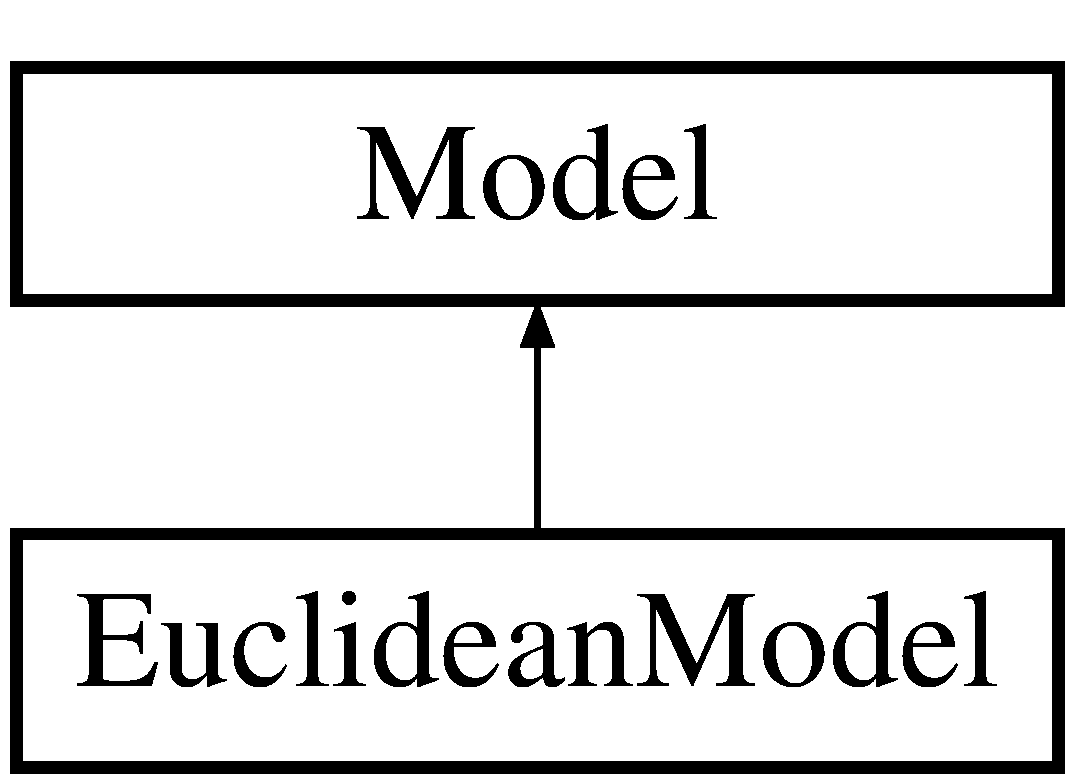
\includegraphics[height=2.000000cm]{classEuclideanModel}
\end{center}
\end{figure}
\subsection*{Public Member Functions}
\begin{DoxyCompactItemize}
\item 
\hypertarget{classEuclideanModel_ab8ab5c07885267649b3b209580df4987}{}void {\bfseries Set\+Max} (double $\ast$p\+\_\+max)\label{classEuclideanModel_ab8ab5c07885267649b3b209580df4987}

\item 
\hypertarget{classEuclideanModel_aea454d5970238c76484d64a582262bfe}{}double $\ast$ {\bfseries Get\+Max} ()\label{classEuclideanModel_aea454d5970238c76484d64a582262bfe}

\item 
\hypertarget{classEuclideanModel_a0dc92790300467bf9c0de80deea99f1b}{}void {\bfseries Set\+Min} (double $\ast$p\+\_\+min)\label{classEuclideanModel_a0dc92790300467bf9c0de80deea99f1b}

\item 
\hypertarget{classEuclideanModel_a4c37d253d3c22746b29dc9aec1c3a982}{}double $\ast$ {\bfseries Get\+Min} ()\label{classEuclideanModel_a4c37d253d3c22746b29dc9aec1c3a982}

\item 
\hypertarget{classEuclideanModel_a47ac11e9db0c00f0f33b129ce130a23e}{}void {\bfseries Set\+Threshold} (double p\+\_\+thres)\label{classEuclideanModel_a47ac11e9db0c00f0f33b129ce130a23e}

\item 
\hypertarget{classEuclideanModel_a5198642a71088c7a8213aba2d3da7e4b}{}double {\bfseries Get\+Threshold} ()\label{classEuclideanModel_a5198642a71088c7a8213aba2d3da7e4b}

\item 
\hypertarget{classEuclideanModel_a64bee90910044ea9072b5b94729e690b}{}void {\bfseries Set\+Avg\+Dst} (double p\+\_\+avg\+\_\+dst)\label{classEuclideanModel_a64bee90910044ea9072b5b94729e690b}

\item 
\hypertarget{classEuclideanModel_a87567dde151b28378135ac0bb2fbdbe0}{}double {\bfseries Get\+Avg\+Dst} ()\label{classEuclideanModel_a87567dde151b28378135ac0bb2fbdbe0}

\item 
\hypertarget{classEuclideanModel_a9e6d476b458300bbb30fc95b1b3be833}{}void {\bfseries Set\+Dvt} (double p\+\_\+dvt)\label{classEuclideanModel_a9e6d476b458300bbb30fc95b1b3be833}

\item 
\hypertarget{classEuclideanModel_ad2597398fd70d06c618c1016f405400c}{}double {\bfseries Get\+Dvt} ()\label{classEuclideanModel_ad2597398fd70d06c618c1016f405400c}

\item 
\hypertarget{classEuclideanModel_ae1ca5081ea838fa22a3f3cfa72733314}{}void {\bfseries Set\+Average} (\hyperlink{classMatrix}{Matrix} $\ast$p\+\_\+avg)\label{classEuclideanModel_ae1ca5081ea838fa22a3f3cfa72733314}

\item 
\hypertarget{classEuclideanModel_a66348bde76d72283320e8f9bd5d8c050}{}\hyperlink{classMatrix}{Matrix} $\ast$ {\bfseries Get\+Average} ()\label{classEuclideanModel_a66348bde76d72283320e8f9bd5d8c050}

\item 
\hypertarget{classEuclideanModel_afb865b54e2ec6fddaa7da4779f469d25}{}void {\bfseries Set\+Num\+Elements} (int p\+\_\+num\+\_\+elements)\label{classEuclideanModel_afb865b54e2ec6fddaa7da4779f469d25}

\item 
\hypertarget{classEuclideanModel_a3a548846f3eb38ff60a0883e384f63cb}{}int {\bfseries Get\+Num\+Elements} ()\label{classEuclideanModel_a3a548846f3eb38ff60a0883e384f63cb}

\item 
\hypertarget{classEuclideanModel_a185afd6127fd323ca4e6f9b0761cc1be}{}void {\bfseries Inc\+Num\+Avg\+Elements} ()\label{classEuclideanModel_a185afd6127fd323ca4e6f9b0761cc1be}

\item 
\hypertarget{classEuclideanModel_a292c72827159ab3c47b1a965974fc54f}{}int {\bfseries Get\+Num\+Avg\+Elements} ()\label{classEuclideanModel_a292c72827159ab3c47b1a965974fc54f}

\item 
\hypertarget{classEuclideanModel_ad090ab6a2e2d1a01b6b986d103300f78}{}void {\bfseries Inc\+Num\+Thr\+Elements} ()\label{classEuclideanModel_ad090ab6a2e2d1a01b6b986d103300f78}

\item 
\hypertarget{classEuclideanModel_a6893e6d8a11314d8b3142d5c6d07ba4b}{}int {\bfseries Get\+Num\+Thr\+Elements} ()\label{classEuclideanModel_a6893e6d8a11314d8b3142d5c6d07ba4b}

\item 
\hypertarget{classEuclideanModel_abfdc672a34b5e030be035b046b981d66}{}void {\bfseries Reset} ()\label{classEuclideanModel_abfdc672a34b5e030be035b046b981d66}

\end{DoxyCompactItemize}
\subsection*{Friends}
\begin{DoxyCompactItemize}
\item 
\hypertarget{classEuclideanModel_ac933d15ad4b493f033e627ac7c7b6157}{}std\+::ostream \& {\bfseries operator$<$$<$} (std\+::ostream \&s, \hyperlink{classEuclideanModel}{Euclidean\+Model} \&p)\label{classEuclideanModel_ac933d15ad4b493f033e627ac7c7b6157}

\end{DoxyCompactItemize}


\subsection{Detailed Description}
Euclidian model for the 1st algorithm for A\+D Inherit from \hyperlink{classModel}{Model}. 

The documentation for this class was generated from the following file\+:\begin{DoxyCompactItemize}
\item 
\hyperlink{ads-simulator_8cc}{ads-\/simulator.\+cc}\end{DoxyCompactItemize}

\hypertarget{classMatrix}{}\section{Matrix Class Reference}
\label{classMatrix}\index{Matrix@{Matrix}}


Tool class used for manipulate data from input data and features.  


\subsection*{Public Member Functions}
\begin{DoxyCompactItemize}
\item 
\hypertarget{classMatrix_af69aee84af5e2c1851eabd46ec65fc59}{}{\bfseries Matrix} (int i, int j)\label{classMatrix_af69aee84af5e2c1851eabd46ec65fc59}

\item 
\hypertarget{classMatrix_a3ce72ec14cb358b23ea14549b8816e4a}{}{\bfseries Matrix} (int i, int j, double $\ast$$\ast$matrix)\label{classMatrix_a3ce72ec14cb358b23ea14549b8816e4a}

\item 
\hypertarget{classMatrix_a353d02e26bafa481d00e866e39e21a41}{}double {\bfseries Get} (int i, int j)\label{classMatrix_a353d02e26bafa481d00e866e39e21a41}

\item 
\hypertarget{classMatrix_a4258bd5497e81af8ea908338dbe83664}{}void {\bfseries Set} (int i, int j, double value)\label{classMatrix_a4258bd5497e81af8ea908338dbe83664}

\item 
\hypertarget{classMatrix_a31f81a2b114be86717ce1aa91bc10cfd}{}double $\ast$ {\bfseries Get\+Column} (int j)\label{classMatrix_a31f81a2b114be86717ce1aa91bc10cfd}

\item 
\hypertarget{classMatrix_afceacf07aff7ed4c3b9ae9dc761e7135}{}int {\bfseries Get\+Size\+I} ()\label{classMatrix_afceacf07aff7ed4c3b9ae9dc761e7135}

\item 
\hypertarget{classMatrix_a642b9a4e1c982ac40477dd8c8b1eae10}{}int {\bfseries Get\+Size\+J} ()\label{classMatrix_a642b9a4e1c982ac40477dd8c8b1eae10}

\item 
\hypertarget{classMatrix_ab97e4bd28c3a93277702a6d21212ecbb}{}\hyperlink{classMatrix}{Matrix} $\ast$ {\bfseries calculate\+Median} ()\label{classMatrix_ab97e4bd28c3a93277702a6d21212ecbb}

\end{DoxyCompactItemize}
\subsection*{Friends}
\begin{DoxyCompactItemize}
\item 
\hypertarget{classMatrix_a5ac1143f9f2df2f556d21e1f16891b52}{}std\+::ostream \& {\bfseries operator$<$$<$} (std\+::ostream \&s, \hyperlink{classMatrix}{Matrix} \&p)\label{classMatrix_a5ac1143f9f2df2f556d21e1f16891b52}

\end{DoxyCompactItemize}


\subsection{Detailed Description}
Tool class used for manipulate data from input data and features. 

The documentation for this class was generated from the following file\+:\begin{DoxyCompactItemize}
\item 
\hyperlink{ads-simulator_8cc}{ads-\/simulator.\+cc}\end{DoxyCompactItemize}

\hypertarget{classModel}{}\section{Model Class Reference}
\label{classModel}\index{Model@{Model}}


Abstract class of \hyperlink{classModel}{Model}.  


Inheritance diagram for Model\+:\begin{figure}[H]
\begin{center}
\leavevmode
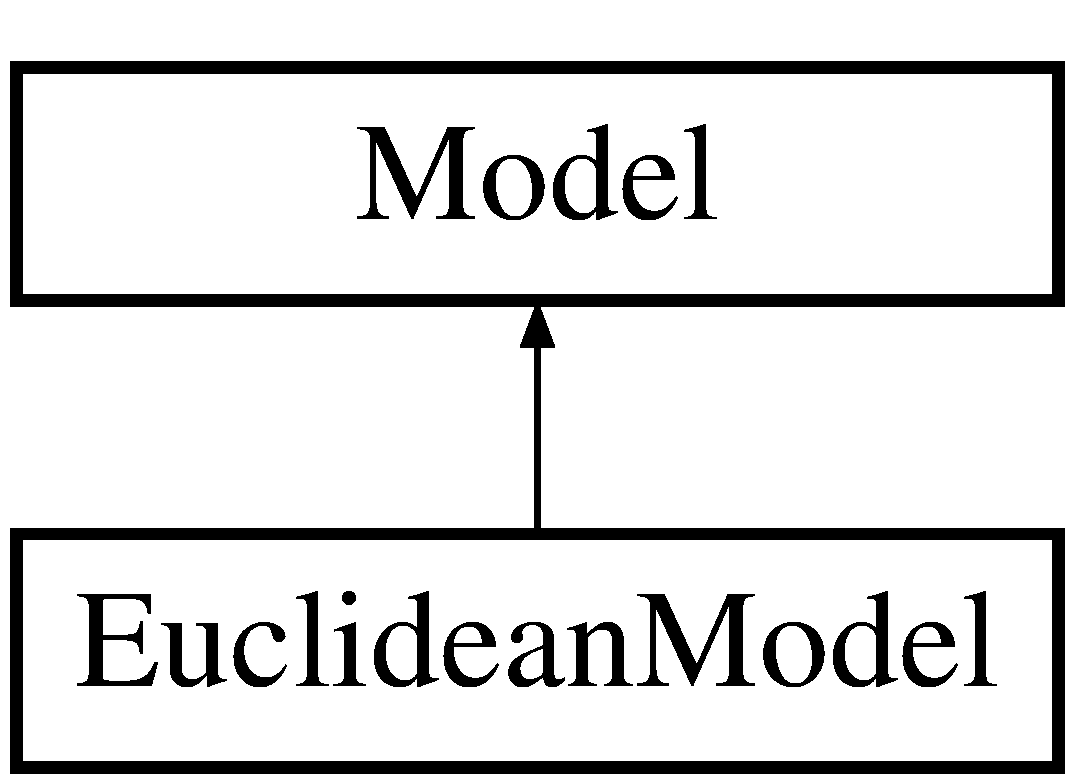
\includegraphics[height=2.000000cm]{classModel}
\end{center}
\end{figure}


\subsection{Detailed Description}
Abstract class of \hyperlink{classModel}{Model}. 

The documentation for this class was generated from the following file\+:\begin{DoxyCompactItemize}
\item 
\hyperlink{ads-simulator_8cc}{ads-\/simulator.\+cc}\end{DoxyCompactItemize}

\hypertarget{structResult}{}\section{Result Struct Reference}
\label{structResult}\index{Result@{Result}}
\subsection*{Public Attributes}
\begin{DoxyCompactItemize}
\item 
\hypertarget{structResult_a33ea1264dd1da37c4f4b0396febeee09}{}bool {\bfseries decision}\label{structResult_a33ea1264dd1da37c4f4b0396febeee09}

\item 
\hypertarget{structResult_a88d8b02b90ea30990ae18709d0cf389d}{}double {\bfseries believe}\label{structResult_a88d8b02b90ea30990ae18709d0cf389d}

\item 
\hypertarget{structResult_a56c15ef50579a0eb5495a42f6f5c3faa}{}Attack\+Type {\bfseries attack}\label{structResult_a56c15ef50579a0eb5495a42f6f5c3faa}

\end{DoxyCompactItemize}


The documentation for this struct was generated from the following file\+:\begin{DoxyCompactItemize}
\item 
\hyperlink{ads-simulator_8cc}{ads-\/simulator.\+cc}\end{DoxyCompactItemize}

\chapter{File Documentation}
\hypertarget{ads-simulator_8cc}{}\section{ads-\/simulator.cc File Reference}
\label{ads-simulator_8cc}\index{ads-\/simulator.\+cc@{ads-\/simulator.\+cc}}


File containing the A\+D detector and simulation This file contains both headers and declarations for classes + run the simulator in the main class (instead of classic couple .h and .cc because I need to understand the setup to do so in N\+S3 (act as module or similar with wscript).  


{\ttfamily \#include \char`\"{}ns3/core-\/module.\+h\char`\"{}}\\*
{\ttfamily \#include $<$math.\+h$>$}\\*
{\ttfamily \#include \char`\"{}ns3/node.\+h\char`\"{}}\\*
\subsection*{Classes}
\begin{DoxyCompactItemize}
\item 
struct \hyperlink{structResult}{Result}
\item 
class \hyperlink{classMatrix}{Matrix}
\begin{DoxyCompactList}\small\item\em Tool class used for manipulate data from input data and features. \end{DoxyCompactList}\item 
class \hyperlink{classModel}{Model}
\begin{DoxyCompactList}\small\item\em Abstract class of \hyperlink{classModel}{Model}. \end{DoxyCompactList}\item 
class \hyperlink{classDataSource}{Data\+Source}
\begin{DoxyCompactList}\small\item\em Abstract class of \hyperlink{classDataSource}{Data\+Source}. \end{DoxyCompactList}\item 
class \hyperlink{classDetector}{Detector}
\begin{DoxyCompactList}\small\item\em Abstract class of \hyperlink{classDetector}{Detector}. \end{DoxyCompactList}\item 
class \hyperlink{classEuclideanModel}{Euclidean\+Model}
\begin{DoxyCompactList}\small\item\em Euclidian model for the 1st algorithm for A\+D Inherit from \hyperlink{classModel}{Model}. \end{DoxyCompactList}\item 
class \hyperlink{classDetectorEuclidean}{Detector\+Euclidean}
\begin{DoxyCompactList}\small\item\em Euclidian detector used for the 1st algorithm for A\+D Inherit from \hyperlink{classDetector}{Detector}. \end{DoxyCompactList}\end{DoxyCompactItemize}
\subsection*{Enumerations}
\begin{DoxyCompactItemize}
\item 
\hypertarget{ads-simulator_8cc_a904b2f9c8f3951116c343784c59d6afe}{}enum {\bfseries Attack\+Type} \{ \\*
{\bfseries A\+T\+\_\+\+D\+R\+A\+I\+N}, 
{\bfseries A\+T\+\_\+\+D\+R\+A\+I\+N\+\_\+\+M\+I\+T}, 
{\bfseries A\+T\+\_\+\+G\+R\+E\+Y\+H\+O\+L\+E}, 
{\bfseries A\+T\+\_\+\+G\+R\+E\+Y\+H\+O\+L\+E\+\_\+\+M\+I\+T}, 
\\*
{\bfseries A\+T\+\_\+\+F\+L\+O\+O\+D}, 
{\bfseries A\+T\+\_\+\+F\+L\+O\+O\+D\+\_\+\+M\+I\+T}, 
{\bfseries A\+T\+\_\+\+M\+A\+X\+N\+U\+M}
 \}\label{ads-simulator_8cc_a904b2f9c8f3951116c343784c59d6afe}

\end{DoxyCompactItemize}
\subsection*{Functions}
\begin{DoxyCompactItemize}
\item 
\hypertarget{ads-simulator_8cc_a796f987c7a114e4a30f99022fac1af0d}{}{\bfseries N\+S\+\_\+\+L\+O\+G\+\_\+\+C\+O\+M\+P\+O\+N\+E\+N\+T\+\_\+\+D\+E\+F\+I\+N\+E} (\char`\"{}A\+D\+S\+Simulator\char`\"{})\label{ads-simulator_8cc_a796f987c7a114e4a30f99022fac1af0d}

\item 
\hypertarget{ads-simulator_8cc_a0ddf1224851353fc92bfbff6f499fa97}{}int {\bfseries main} (int argc, char $\ast$argv\mbox{[}$\,$\mbox{]})\label{ads-simulator_8cc_a0ddf1224851353fc92bfbff6f499fa97}

\end{DoxyCompactItemize}


\subsection{Detailed Description}
File containing the A\+D detector and simulation This file contains both headers and declarations for classes + run the simulator in the main class (instead of classic couple .h and .cc because I need to understand the setup to do so in N\+S3 (act as module or similar with wscript). 


%--- End generated contents ---

% Index
\backmatter
\newpage
\phantomsection
\clearemptydoublepage
\addcontentsline{toc}{chapter}{Index}
\printindex

\end{document}
